%% ID: the_hosepipe
%% TITLE: The Hosepipe
%% TYPE: question
%% QUESTIONTYPE: numeric
%% CONCEPTS: momentum, newtonii, friction, resolving_vectors, vectors
%% VIDEOS: 
%% LEVEL: 5
%% TOPIC: mechanics/dynamics
%% ORDER: 7

\begin{problem}[HSC1931MIIIQ3pa] % metric units added
{\exposition{A hose pipe delivers a jet of water \valuedef{d}{2}{cm} in diameter, which impinges horizontally and normally on a side of a box weighing \valuedef{m}{1}{kg}, whose base rests in contact with a rough horizontal floor; the coefficient of friction between the box and floor is \valuedef{\mu}{\frac{1}{2}}{}.}  \question{Assuming that the water is of density \valuedef{\rho}{1000}{kg\,m\sup{-3}} and does not recoil from the box, determine the smallest velocity of the jet that will cause the box to move.}}
{\stress{Adapted with permission from UCLES, Higher School Certificate Mathematics, June~1931, Paper~3, Question~3.}}
{As always, a diagram is the first step to solving the problem; as in Figure \ref{fig:Dynamics_water_jet_block}.

\begin{figure}[h]
	\centering
	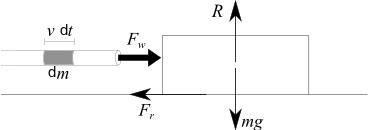
\includegraphics[width=0.5\textwidth]{../../../figures/Dynamics_water_jet_block.svg}
	\caption{}
	\label{fig:Dynamics_water_jet_block}
\end{figure}

The force the water exerts on the block, \vari{F_{w}}, is that from the change in momentum of the water as it hits the block; which, since the water does not recoil, must be all of its horizontal momentum. Using Newton's Second Law, \valuedef{\vtr{F}}{\frac{\d\vtr{p}}{\d t}}{}, we can find the force by considering an element of the water jet:
\begin{equation*} 
\d p = v \d m 
\end{equation*}

Considering an element of the jet, in a time \vari{\d t} a mass \valuedef{\d m}{A\rho v\d t}{} is delivered, where \vari{A} is the cross sectional area of the jet: \valuedef{A}{\frac{1}{4}\pi d^{2}}{}. This follows because the length of the element is \vari{v \d t} and the area is \vari{A}, giving a volume of \vari{A v \d t} and so a mass of \vari{A \rho v \d t}.
\begin{align*} 
\d m & = A \rho v \d t \\ 
&= \left(\frac{1}{4}\pi d^{2}\right) \rho v \d t \\
 &= \frac{1}{4} \pi \rho v d^{2} \d t 
 \end{align*}
so then the momentum of that element \vari{\d p} is simply:
\begin{align*} 
\d p &= \frac{1}{4}\pi\rho v^{2} d^{2} \d t 
\end{align*}

This allows us to find \vari{\frac{\d p}{\d t}} and hence the force from the water:
\begin{align*} 
\frac{\d p}{\d t} &= \frac{1}{4}\pi\rho v^{2} d^{2} \frac{\d t}{\d t} \\ 
&= \frac{1}{4}\pi\rho v^{2} d^{2} \\ 
&= F_{w}
 \end{align*}

The block will accelerate when \vari{F_{w}} $>$ \vari{F_{r}}, but the minimum velocity will be when they are equal and friction is at a maximum:
\begin{align*} 
F_{w} &= F_{r} \\ &= \mu R \\ 
&= \mu mg \\
 \frac{1}{4}\pi\rho v^{2} d^{2} &= \mu mg \\
  v^{2} &= \frac{4\mu mg}{\pi\rho d^{2}} \\ 
  v &= \sqrt{\frac{4\mu mg}{\pi\rho d^{2}}}
  \end{align*}
Substituting in the numbers from the question:
\begin{align*}
 v &= \sqrt{\frac{4\left(\frac{1}{2}\right)(1)(9.8)}{\pi(1000)(0.02)^{2}}}  \\ 
 \anwer{v &\approx \mbox{\quantity{3.95}{m\,s\sup{-1}}}}
  \end{align*}
}
\end{problem}